\documentclass{beamer}

\usepackage[T2A]{fontenc}
\usepackage[utf8]{inputenc}
\usepackage[english,russian]{babel}
\usepackage{amssymb,amsfonts,amsmath,mathtext}
\usepackage{cite,enumerate,float,indentfirst}

\usepackage{graphicx}
\usepackage{booktabs}
\usepackage{tabularx}

\usepackage{qtree}    % regular trees (e.g. GB style)
\usepackage{gb4e}     % numbered lists for linguistic examples

\usepackage{caption}
\captionsetup{font=scriptsize}

% CCG parse trees
\newcommand{\deriv}[2]
{  \renewcommand{\arraystretch}{.5}
	$\begin{array}[t]{*{#1}{c}}
	#2
	\end{array}$ }
\newcommand{\gf}[1]{\textsf{\textsl{#1}}}
\newcommand{\cf}[1]{\mbox{\ensuremath{\cfont{#1}}}}
\newcommand{\uline}[1]
{\mc{#1}{\hrulefill} }
\newcommand{\mc}[2]
{\multicolumn{#1}{c}{#2}}
\newcommand{\cfont}{\mathsf}
\newcommand{\bs}{\backslash}
\newcommand{\subsa}[1]{\hspace{-0.75mm}_{_{#1}}}
\newcommand{\subsb}[1]{\hspace{-0.10mm}_{_{#1}}}
\newcommand{\subs}[1]{\hspace{-0.40mm}_{#1}}
\newcommand{\subsf}[1]{\hspace{-0.75mm}_{_{#1}}}
\newcommand{\supsa}[1]{\hspace{-1.75mm}^{^{#1}} }
\newcommand{\supsb}[1]{\hspace{-0.80mm}^{^{#1}}  }
\newcommand{\sups}[1]{\hspace{-0.40mm}^{#1}}

\graphicspath{{images/}}

\usetheme{Rochester}
\usecolortheme{seagull}

\setbeamertemplate{footline}{\scriptsize{\hspace*{0.4cm}\insertframenumber}\vspace*{0.3cm}}
\beamertemplatenavigationsymbolsempty

\errorcontextlines 10000

\begin{document}

\title{\large{\sc Язык как объект моделирования}}
\author{Константин Соколов}
%\institute[]{СПбГПУ}
%\date{Санкт-Петербург, 2015} 

\begin{frame}
    \thispagestyle{empty}
    \titlepage
\end{frame}

 

\begin{frame}{}
\begin{itemize}
	\item Письменность и Unicode
	\item Уровневая теория языка
	\item Неоднозначность
\end{itemize}
\end{frame}
 
%%%%%%%%%%%%%%%%%%%%%%%%%%%%
% 1. Письменность
%%%%%%%%%%%%%%%%%%%%%%%%%%%%

\begin{frame}{}
\begin{center}
	\textbf{Письменность}
\end{center}
\end{frame}

%     алфавитное и слоговое письмо, иероглифика; 
\begin{frame}{Алфавит}
\begin{figure}[H]
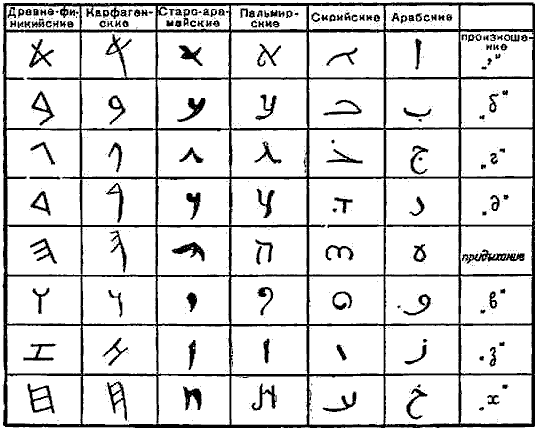
\includegraphics[scale=0.4]{alphabet.png} 
\end{figure}
\end{frame}

\begin{frame}{Слоговое письмо}
\begin{figure}[H]
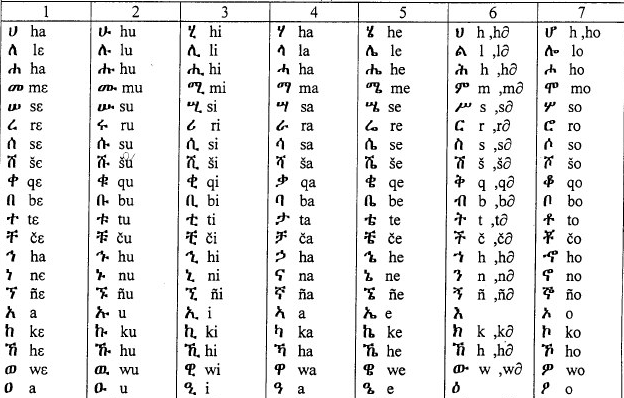
\includegraphics[scale=0.45]{amharic.png} 
\end{figure}
\end{frame}

\begin{frame}{Идеографическое письмо}
\begin{figure}[H]
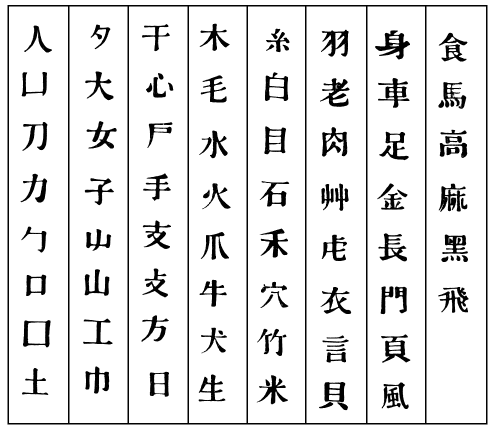
\includegraphics[scale=0.6]{ideographic.png} 
\end{figure}
\end{frame}

% ктив мале и ктив хасер; огласовки
\begin{frame}{Никуд}
\begin{figure}[H]

\includegraphics[scale=0.6]{hebrew.png} 
\end{figure}
\end{frame}

% направление письма
\begin{frame}{Двунаправленные тексты}
\begin{figure}[H]
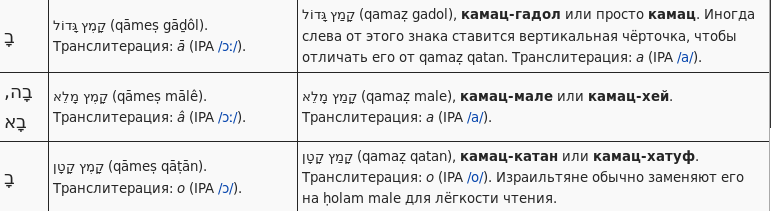
\includegraphics[scale=0.4]{bidirectional.png} 
\end{figure}
\end{frame}

% катакана, хирагана, кандзи, ромадзи
\begin{frame}{Кана}
\begin{figure}[H]
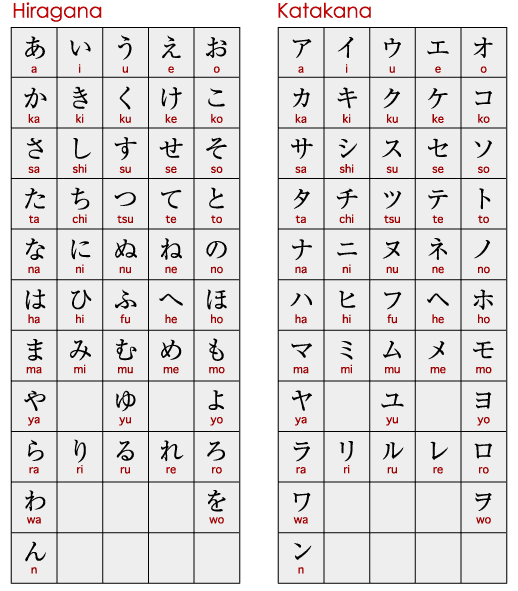
\includegraphics[scale=0.35]{kana.png} 
\end{figure}
\end{frame}

\begin{frame}{Кандзи}
\begin{figure}[H]
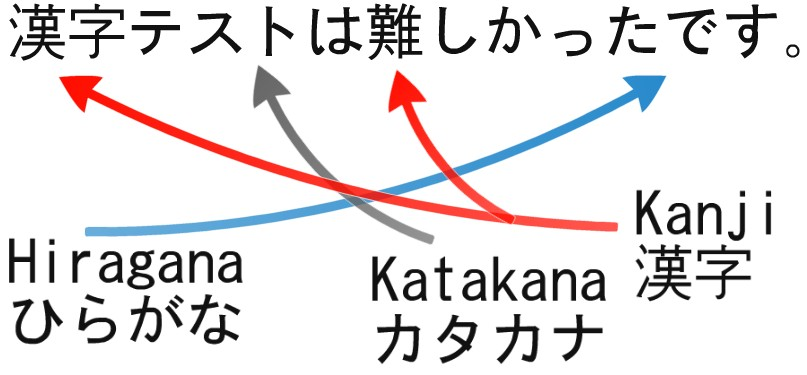
\includegraphics[scale=0.3]{kanji.jpg} 
\end{figure}
\end{frame}

%   диакритика 
\begin{frame}{Диакритика}
\begin{figure}[H]
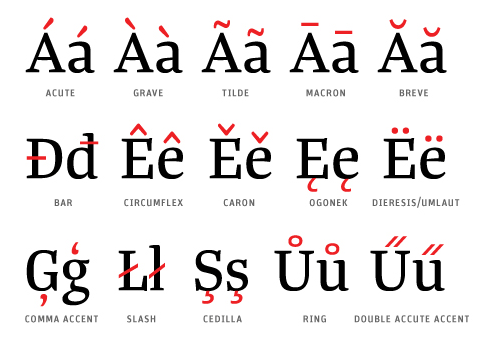
\includegraphics[scale=0.45]{diacritic.png} 
\end{figure}
\end{frame}

% лигатуры
\begin{frame}{Лигатуры (I)}
\begin{figure}[H]
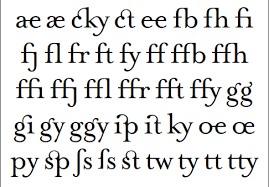
\includegraphics[scale=0.8]{ligatura.png} 
\end{figure}
\end{frame}

\begin{frame}{Лигатуры (II)}
\begin{figure}[H]

\includegraphics[scale=0.5]{devanagari.png} 
\end{figure}
\end{frame}

\begin{frame}{}
\begin{center}
\textbf{Unicode}
\end{center}
\end{frame}

\begin{frame}{Графема}
\begin{itemize}
\item аллограф (начертание) и графема
\item глиф (glyph) и код (code point)
	\begin{itemize}
		\item примеры глифов: буквы (вкл. позиционные варианты), знаки препинания, акценты, огласовки, лигатуры и пр.
		\item один аллограф может включать несколько глифов
		\item пример code point: \texttt{U+0639} (hex)
	\end{itemize}
\end{itemize}
\bigskip
\begin{figure}[H]
	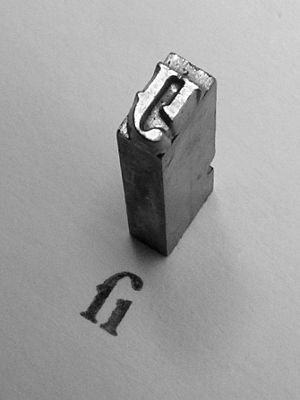
\includegraphics[scale=0.2]{glyph.jpg} 
	\caption*{Глиф -- отдельный графический элемент}
\end{figure}
\end{frame}

% Unicode, представление диакритики в Unicode, нормализация Unicode); ICU (http://site.icu-project.org/)
\begin{frame}{Unicode (I)}
Необходимо различать три понятия:\\
\bigskip
\begin{itemize}
\item character set -- неупорядоченный набор графических элементов
\item coded character set -- набор кодов (абстрактных числовых идентификаторов графем)
\item character encoding scheme -- кодировка (байтовое представление кодов)
\end{itemize}
\end{frame}

\begin{frame}{Unicode (II)}
combining characters -- глиф может образовываться с помощью базового символа и модификаторов\\
\medskip
\begin{figure}[H]
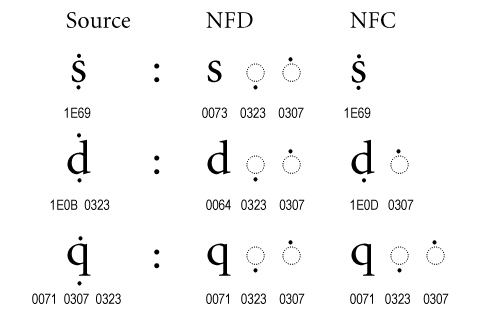
\includegraphics[scale=0.4]{combining.png} 
\end{figure}
\end{frame}

\begin{frame}{Unicode (III)}
\begin{figure}[H]
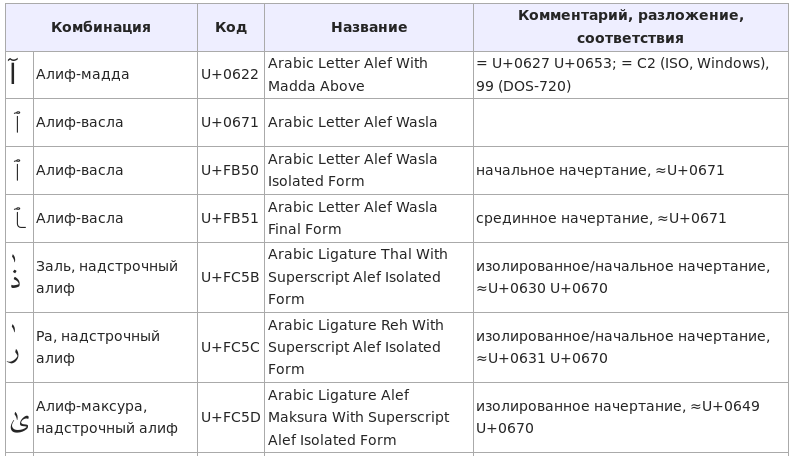
\includegraphics[scale=0.35]{combining-arabic.png} 
\end{figure}
\end{frame}

\begin{frame}{Unicode (IV)}
\begin{itemize}
\item collation -- ``сортировка''
\begin{itemize}
\item в испанском диграф \textit{ch} трактуется как одна буква \textit{(c, ch, d)}
\item \textit{\'{e}} может считаться эквивалентным \textit{e}
\item в немецком \textit{\"{a}} и \textit{ae} могут считаться эквивалентными
\item разный алфавитный порядок (лит.: \textit{i, y, k}; англ.: \textit{i, j, k})
\end{itemize}	
\medskip
\item кодировка
\begin{itemize}
\item UCS-2: 2 байта на code point 
\item UTF-8: 1 байт для символов с code points < 127 (совпадает с ASCII), всего до 6 байтов на code point
\item Byte Order Mark (\texttt{FF\,EF} vs. \texttt{EF\,FF})
\end{itemize}	
\end{itemize}
\end{frame}

\begin{frame}{Нормализация Unicode (I)}
\begin{itemize}
\item Unicode Normalization Forms 
\begin{itemize}
\item \texttt{http://www.unicode.org/reports/tr15}
\end{itemize} 
\medskip
\item Два вида эквивалентности последовательностей символов
\begin{itemize}
\item canonical equivalence (напр., различные способы упорядочить модификаторы)
\item compatibility equivalence (напр., различные варианты, вкл. позиционные)
\end{itemize} 
\end{itemize}
\end{frame}

\begin{frame}{Нормализация Unicode (II)}
\begin{itemize}
\item Нормальные формы определяются на основе композиции и декомпозиции code points
\begin{itemize}
\item NFD (Normalization Form D) -- каноническая декомпозиция
\item NFC -- каноническая декомпозиция, затем каноническая композиция
\item NFKD -- совместимая декомпозиция
\item NFKC -- совместимая декомпозиция, затем совместимая композиция
\end{itemize} 
\end{itemize}
\end{frame}

\begin{frame}{Нормализация Unicode (III)}
\begin{figure}[H]
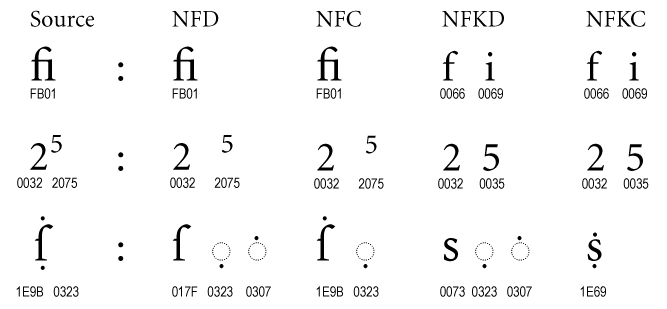
\includegraphics[scale=0.4]{normalized.png} 
\end{figure}
\end{frame}

 
 
 
 
%%%%%%%%%%%%%%%%%%%%%%%%%
% 2. Уровневая теория
%%%%%%%%%%%%%%%%%%%%%%%%%

\begin{frame}{}
\begin{center}
	\textbf{Уровневая теория}
\end{center}
\end{frame}

% уровневая теория, понятие интерфейса 
\begin{frame}{Уровни языка (I)}
\setcounter{framenumber}{1}
\begin{itemize}
    \item уровни языка -- автономные ярусы языковой системы
    	\begin{itemize}
			\item лексикон
			\item фонология
			\item морфология
			\item синтаксис
			\item семантика    	
    	\end{itemize}
	\item предпосылка выделения уровней -- формальное моделирование (определение единиц уровня, критериев их разграничения)    	
\end{itemize}
\end{frame}

\begin{frame}{Уровни языка (II)}
\begin{itemize}
	\item уровни оперируют однородными единицами
	\item единицы одного уровня способны вступать в синтагматические и парадигматические отношения (слова -- словосочетания)
	\item единицы разных уровней способны вступать в иерархические отношения (фонемы -- морфемы -- словоформы)
	\item эмические (фонемы, морфемы) и этические (фоны, морфы) единицы 
\end{itemize}
\end{frame}

\begin{frame}{Уровни языка (III)}
\begin{itemize}
	\item интерфейсы 
	    \begin{itemize}
	    	\item фонолого-морфологический
	    	\item морфолого-синтаксический
	    	\item синтактико-семантический
	    \end{itemize}
\end{itemize}
\end{frame}

\begin{frame}{}
\begin{center}
	\textit{Трудности определения границ языковых уровней \\на примере морфологии}
\end{center}
\end{frame}

\begin{frame}{Типы языков -- I}
Натуралистическая концепция языка (А.~Шлейхер, 1821 -- 1868)\\
\medskip
\begin{itemize}
\item изолирующие
\item агглютинативные
\item флективные древние
\item флективные новые (аналитические)
\end{itemize}
\end{frame}

\begin{frame}{Типы языков -- II}
Изолирующие языки\\
\medskip
\begin{itemize}
\item аморфные, односложные, корневые
\item языки Юго-Восточной Азии
\item \textit{t\={a}men z\`{a}i zu\`{o} zu\`{o}y\`{e}} (они НАСТ делать уроки) (кит.)
\end{itemize}
\end{frame}

\begin{frame}{Типы языков -- III}
Агглютинативные языки\\
\medskip
\begin{itemize}
\item формы образуются путем присоединения аффиксов 
\item аффиксы однозначны, их границы легко различимы
\item алтайские, финно-угорские, тюркские
\item узбекский: \textit{китоб} (книга), \textit{китоблар} (книги),\\ \textit{китобларда} (в книгах)
\end{itemize}
\end{frame}

\begin{frame}{Типы языков -- IV}
Флективные языки\\
\medskip
\begin{itemize}
\item флексии сочетают несколько значений, границы размыты
\item фузия -- фонетические изменения на стыках морфем
\item индоевропейские, семитские
\item \textit{стричь} (стриг- + т') (рус.), \textit{dens, dentis} (edo, edens) (лат.)
\end{itemize}
\end{frame}

\begin{frame}{Типы языков -- V}
Аналитические языки\\
\medskip
\begin{itemize}
\item грамматические отношения выражаются служебными словами, порядком слов, интонацией и т. п., а не словоизменением
\item новоевропейские (английский, французский, африкаанс)
\item \textit{he will kiss me} (англ.) vs. \textit{yena\v{s}keni} (иврит)
\end{itemize}
\end{frame}

\begin{frame}{Линейно-синтагматическая сочетаемость}
\begin{itemize}
\item языковой дрейф (Э. Сепир, 1921)
\item словоформа, морфема, аффикс
\item морфема и алломорф
\end{itemize}
\end{frame}

\begin{frame}{Корни и аффиксы}
Неконкатенативная морфология\\
\medskip
\begin{itemize}
\item аблаут (\textit{foot -- feet})
\item трансфиксация (\textit{l\={a}mad -- l\={o}med -- yilm\={o}d, limud, melamed})
\item редупликация (\textit{чуть-чуть, белым-бело})
\end{itemize}
\end{frame}

\begin{frame}{Модели морфологии}
\begin{itemize}
\item элементно-комбинаторные (Item and Arrangement, IA)
\item элементно-операционные (Item and Process, IP)
\item словесно-парадигматические (Word and Paradigm, WP)
\end{itemize}
\end{frame}




%%%%%%%%%%%%%%%%%%%%%%%%
% 2. Неоднозначность
%%%%%%%%%%%%%%%%%%%%%%%%

\begin{frame}{}
\begin{center}
	\textbf{Неоднозначность}
\end{center}
\end{frame}

\begin{frame}{Омонимы}
\begin{itemize}
\item полные омонимы
\begin{itemize}
\item \textit{ручка} (для письма) -- \textit{ручка} (маленькая рука)
\item \textit{наряд} (одежда) -- \textit{наряд} (распоряжение)
\end{itemize}
\item частичные омонимы
\begin{itemize}
\item \textit{ласка} (зверь) -- \textit{ласка} (действие), но \textit{ласок} (р.п., мн.ч.), \textit{ласк} (р.п., мн.ч.)
\end{itemize}
\item грамматические (совпадение отдельных форм)
\begin{itemize}
\item \textit{к трём} (часам), \textit{мы трём} (что-то)
\end{itemize}
\end{itemize}
\end{frame}

\begin{frame}{Омографы}
\begin{itemize}
\item разные слова
\begin{itemize}
\item \textit{в\'{о}рон} (м.р., ед.ч., и.п.) -- \textit{вор\'{о}н} (ж.р., мн. ч., р.п.)
\item \textit{м\'{е}сти} (сущ., ж.р., р.п. или п.п.) -- \textit{мест\'{и}} (гл.)
\end{itemize}
\item формы одного слова
\begin{itemize}
\item \textit{б\'{у}дите} -- \textit{буд\'{и}те}
\item \textit{м\'{е}ста} — \textit{мест\'{а}}
\end{itemize}
\end{itemize}
\end{frame}

\begin{frame}{``Паразитная'' омонимия}
\begin{itemize}
\item ``\textit{Махабхарата} получает несколько гипотетических разборов, в том числе от псевдолексем \textit{махабхаронок}, \textit{махабхарать}.'' (с сайта НКРЯ)
\item singularia tantum
\begin{itemize}
\item \textit{еда} (sg.t.), \textit{*\'{е}ды} (мн.ч., и.п.), но \textit{ед\'{ы}} (ед.ч., р.п.)
\end{itemize}
\item pluralia tantum
\begin{itemize}
\item \textit{часы} (pl.t., предмет), ср. \textit{час} (единица времени), мн.ч. \textit{часы}
\item \textit{гр\'{я}зи} (pl.t., курорт), ср. \textit{грязь} (пачкающая субстанция), р.п. \textit{грязи}
\end{itemize}
\end{itemize}
\end{frame}

\begin{frame}{Слова с различной дистрибуцией}
\begin{itemize}
\item \textit{disputare} (ит.) 
\begin{itemize}
\item обсуждать, спорить (disputare una questione -- обсуждать вопрос)
\item оспаривать (disputare la coppa -- бороться за кубок)
\end{itemize}
\item \textit{сидеть} (в тюрьме) -- \textit{сидеть} (на зарплате)
\item разные части речи
\begin{itemize}
\item \textit{water}, \textit{to water}
\item ``Мой дядя самых честных правил, когда не в шутку занемог; [\dots]'' -- \textit{(пунктуация по изданию 1825 г.)}
\end{itemize}
\end{itemize}
\end{frame}

\begin{frame}[fragile]{Cинтаксическая неоднозначность (I)}
\begin{center}
\Tree [.S [.NP [.Det The ] [.N boy ] ] [.VP [.V saw ] [.NP [.Det the ] [.N man ] [.PP [.P with ] [.NP [.Det the ] [.N telescope ] ] ] ] ] ]
\end{center}
\end{frame}

\begin{frame}[fragile]{Cинтаксическая неоднозначность (II)}
\begin{center}
\Tree [.S [.NP [.Det The ] [.N boy ] ] [.VP [.V saw ] [.NP [.Det the ] [.N man ] ] [.PP [.P with ] [.NP [.Det the ] [.N telescope ] ] ] ] ]
\end{center}
\end{frame}

\begin{frame}{Cинтаксическая неоднозначность (III)}
\begin{center}
\deriv{6}{
\gf{включи} & \gf{лампу} & \gf{и} & \gf{подсветку} & \gf{на} & \gf{кухне} \\
\uline{1} & \uline{1} & \uline{1} & \uline{1} & \uline{1} & \uline{1} \\
\cf{s\bs \supsa{-} np/ np} & \cf{np} & \cf{n/ np\bs \subsb{*} np} & \cf{n} & \cf{pp/ \subsa{\diamond} np} & \cf{np} \\
& \mc{2} {\hrulefill_{<}} \\
& \mc{2}{\cf{n/ np}} \\
&&&& \mc{2} {\hrulefill_{>}} \\
&&&& \mc{2}{\cf{pp}} \\
&&&& \mc{2} {\hrulefill_{t\mathbf{ypechange-6}}}\\
&&&& \mc{2}{\cf{n\bs \subsb{*} n}} \\
&&& \mc{3} {\hrulefill_{<}} \\
&&& \mc{3}{\cf{n}} \\
&&& \mc{3} {\hrulefill_{t\mathbf{ypechange-3}}}\\
&&& \mc{3}{\cf{np}} \\
& \mc{5} {\hrulefill_{>}} \\
& \mc{5}{\cf{n}} \\
& \mc{5} {\hrulefill_{t\mathbf{ypechange-4}}}\\
& \mc{5}{\cf{np}} \\
\mc{6} {\hrulefill_{>}} \\
\mc{6}{\cf{s\bs \supsa{-} np}} \\
}
\end{center}
\end{frame}

\begin{frame}{Cинтаксическая неоднозначность (III)}
\begin{center}
\deriv{6}{
\gf{включи} & \gf{лампу} & \gf{и} & \gf{подсветку} & \gf{на} & \gf{кухне} \\
\uline{1} & \uline{1} & \uline{1} & \uline{1} & \uline{1} & \uline{1} \\
\cf{s\bs \supsa{-} np/ np} & \cf{np} & \cf{n/ np\bs \subsb{*} np} & \cf{np} & \cf{pp/ \subsa{\diamond} np} & \cf{np} \\
& \mc{2} {\hrulefill_{<}} \\
& \mc{2}{\cf{n/ np}} \\
&&&& \mc{2} {\hrulefill_{>}} \\
&&&& \mc{2}{\cf{pp}} \\
& \mc{3} {\hrulefill_{>}} \\
& \mc{3}{\cf{n}} \\
&&&& \mc{2} {\hrulefill_{t\mathbf{ypechange-6}}}\\
&&&& \mc{2}{\cf{n\bs \subsb{*} n}} \\
& \mc{5} {\hrulefill_{<}} \\
& \mc{5}{\cf{n}} \\
& \mc{5} {\hrulefill_{t\mathbf{ypechange-4}}}\\
& \mc{5}{\cf{np}} \\
\mc{6} {\hrulefill_{>}} \\
\mc{6}{\cf{s\bs \supsa{-} np}} \\
}
\end{center}
\end{frame}

\begin{frame}{Анафора}
\begin{itemize}
\item[] \textit{Гражданка Иванова}_i попала в \textit{автомобильную аварию}_j, \textit{которая}_{i/j} произошла сегодня утром на улице Ленина. После проведения экспертизы сотрудники ГИБДД признали \textit{её}_{i/j} виновником ДТП. 
\end{itemize}
\end{frame}

% область действия кванторов: every man admires a woman (каждый мужчина восхищается какой-то женщиной, все мужчины восхищаются одной и той же женщиной); каждый получит награду, которую заслуживает
\begin{frame}{Область действия кванторов}
\begin{itemize}
\item Every man admires a woman
\begin{itemize}
\item $\forall x (man(x) \wedge (\exists y . woman(y) \wedge admires(x,y)))$ 
\item $\exists y (woman(y) \wedge \forall x (man(x) \wedge admires(x,y)))$ 
\end{itemize}
\end{itemize}
\end{frame}

\begin{frame}{Чтения \textit{de re} и \textit{de dicto}}
\smallskip
{\footnotesize	
\begin{exe}
\ex de re + резумптивность
\gll Dani yimca et ha-i\v{s}a \v{s}e hu mexapes \textit{ota}\\
Дани найдёт ACC DET-женщину которая он ищет её-ACC\\
\glt Дани найдёт женщину, которую ищет
\ex de dicto + резумптивность
\gll ha-i\v{s}a \v{s}e Dani mexapes \textit{ota} crixa lihyot blondit\\
DET-женщина которая Дани ищет её-ACC должна быть блондинкой\\
\glt Женщина, которую ищет Дани, должна быть блондинкой
\end{exe}		    
}
\end{frame}

% неоднозначный дейксис: Где привратник? -- гневно кричала она. -- Почему никто не подходит к двери?\\ -- К какой двери? -- спросил Лягушонок. [...]\\ -- К этой, конечно! (Пример Падучевой из Алисы в стране чудес)
% de re vs. de dicto: John seeks a unicorn; примеры про резумпцию в иврите; 
% неоднозначность вследствие эллипсиса: John loves his mother and Bill does too.
\begin{frame}{Неоднозначный дейксис}
Коммуникативная неудача (пример Е.~В.~Падучевой):\\
\bigskip
\begin{itemize}
\item[] \textit{-- Где привратник? -- гневно кричала она. -- Почему никто не подходит к двери?}
\item[] \textit{-- К какой двери? -- спросил Лягушонок. [\dots]}
\item[] \textit{-- К этой, конечно!}
\end{itemize}
\end{frame}

\begin{frame}[fragile]{Spurious ambiguity}
\begin{tiny}
\begin{verbatim}
John        loves            Mary                 John         loves          Mary
np          (s\np)/np        np                   np           (s\np)/np      np
--------T>  --------------------->                             ----------------------->
s/(s\np)              s\np                                              s\np
---------------------------->                     -----------------------------<
s                                                  s

John        loves            Mary                 John         loves          Mary 
np          (s\np)/np        np                   np           (s\np)/np     np
--------T>                   ---------T>          ---------T>
s/(s\np)                     s/(s\np)             s/(s\np)
--------------------------B<          -----------------------B>
s\np                                   s/np
----------------------------->                              --------------------------->
s                                                  s

John        loves            Mary                John           loves         Mary
np          (s\np)/np        np                  np             (s\np)/np     np
---------T>         --------T>                   --------T<
s/(s\np)            s/(s\np)                     s\(s/np)
--------------------------B<         ----------------------B>
s\np                                   s/np
-----------------------------<                              ---------------------------<
s                                                  s
\end{verbatim}
\end{tiny}
\end{frame}







\begin{frame}{}
\thispagestyle{empty}
\begin{center}
	{\large Спасибо!}
\end{center}
\end{frame}


\end{document}